\chapter{Implementacija i korisničko sučelje}
		
		
		\section{Korištene tehnologije i alati}
		
			Komunikacija u timu ostvarena je pomoću platforme Discord\footnote{\url{https://discord.com}} koja nudi opcije tekstualnog dopisivanja, glasovnog poziva i videopoziva. U serveru našeg projektnog tima postojalo je nekoliko kanala koji su se bavili različitim temama (back-end, front-end, dokumentacija…) što nam je pomoglo u podjeli posla i filtriranju zadataka. Za izradu UML dijagrama koristili smo se aplikacijom Astah\footnote{\url{https://astah.net}} pomoću koje smo vrlo jednostavno napravili željene dijagrame i time pokazali ideju projektnog zadatka, kao i način rada naše aplikacije. Kao sustav za upravljanje izvornim kodom koristili smo Git\footnote{\url{https://git-scm.com}}. Udaljeni repozitorij projekta dostupan je na web platformi GitHub\footnote{\url{https://github.com}}. \\
Za razvojno okruženje koristili smo Visual Studio Code\footnote{\url{https://code.visualstudio.com}} i IntelliJ IDEA\footnote{\url{https://jetbrains.com/idea}}. VSC nudi široku podršku za jezike i ekstenzije, integraciju s Git-om i različitim alatima i servisima (Docker\footnote{\url{https://docker.com}}) te snimanje koraka za debuggiranje. Također, dolazi s ugrađenom podrškom za JavaScript i TypeScript. IntelliJ IDEA nudi naprednu podršku za pisanje koda (Code Assistance), odličan debugger, refaktoriranje koda te podršku za različite tehnologije (Spring Framework, JavaScript, HTML, CSS, TypeScript, React, SQL) i jezike (Java, Kotlin, Groovy). \\
Klijentska strana aplikacije (\textit{front-end}) napisana je React\footnote{\url{https://react.dev}}-om preko TypeScript\footnote{\url{https://typescriptlang.org}}-a i Vite.js\footnote{\url{https://vitejs.dev}}-om. Material UI\footnote{\url{https://mui.com/material-ui}} je biblioteka React komponenata koja pruža implementaciju Google-ovog Material Design koncepta u React aplikacijama, a fokusiran je na stvaranje dosljednih i intuitivnih korisničkih sučelja.\\
Poslužiteljska strana aplikacije (\textit{back-end}) napisana je u Kotlinu\footnote{\url{https://kotlinlang.org}} koristeći Spring Framework\footnote{\url{https://spring.io/projects/spring-framework}}. Kotlin omogućuje interoperabilnost s jezikom Java\footnote{\url{https://java.com/en}} (može se koristiti zajedno s njim u sklopu istog projekta te koristiti njegove biblioteke). Spring Framework je open-source radni okvir za razvoj aplikacija baziranih na Javi. On implementira inverziju kontrole (IoC), uvođenje ovisnosti (DI), Model-View-Controller (MVC), pristup podacima, sigurnost i Spring Boot. \\
Pokretanje, izvršavanje i puštanje u pogon izvršavaju se preko 3 kontejnera platforme Docker koji pokrivaju najvažnije dijelove aplikacije: back-end, front-end i PostgreSQL bazu podataka. Pri deployment-u projekta koristimo radni okvir Express.js\footnote{\url{https://expressjs.com}} za izgradnju API-ja s Node.js\footnote{\url{https://nodejs.org/en}} radnim okruženjem.

			
			\eject 
		
	
		\section{Ispitivanje programskog rješenja}
			
			\textbf{\textit{dio 2. revizije}}\\
			
			 \textit{U ovom poglavlju je potrebno opisati provedbu ispitivanja implementiranih funkcionalnosti na razini komponenti i na razini cijelog sustava s prikazom odabranih ispitnih slučajeva. Studenti trebaju ispitati temeljnu funkcionalnost i rubne uvjete.}
	
			
			\subsection{Ispitivanje komponenti}
			\textit{Potrebno je provesti ispitivanje jedinica (engl. unit testing) nad razredima koji implementiraju temeljne funkcionalnosti. Razraditi \textbf{minimalno 6 ispitnih slučajeva} u kojima će se ispitati redovni slučajevi, rubni uvjeti te izazivanje pogreške (engl. exception throwing). Poželjno je stvoriti i ispitni slučaj koji koristi funkcionalnosti koje nisu implementirane. Potrebno je priložiti izvorni kôd svih ispitnih slučajeva te prikaz rezultata izvođenja ispita u razvojnom okruženju (prolaz/pad ispita). }
			
			
			
			\subsection{Ispitivanje sustava}
			
			 \textit{Potrebno je provesti i opisati ispitivanje sustava koristeći radni okvir Selenium\footnote{\url{https://www.seleniumhq.org/}}. Razraditi \textbf{minimalno 4 ispitna slučaja} u kojima će se ispitati redovni slučajevi, rubni uvjeti te poziv funkcionalnosti koja nije implementirana/izaziva pogrešku kako bi se vidjelo na koji način sustav reagira kada nešto nije u potpunosti ostvareno. Ispitni slučaj se treba sastojati od ulaza (npr. korisničko ime i lozinka), očekivanog izlaza ili rezultata, koraka ispitivanja i dobivenog izlaza ili rezultata.\\ }
			 
			 \textit{Izradu ispitnih slučajeva pomoću radnog okvira Selenium moguće je provesti pomoću jednog od sljedeća dva alata:}
			 \begin{itemize}
			 	\item \textit{dodatak za preglednik \textbf{Selenium IDE} - snimanje korisnikovih akcija radi automatskog ponavljanja ispita	}
			 	\item \textit{\textbf{Selenium WebDriver} - podrška za pisanje ispita u jezicima Java, C\#, PHP koristeći posebno programsko sučelje.}
			 \end{itemize}
		 	\textit{Detalji o korištenju alata Selenium bit će prikazani na posebnom predavanju tijekom semestra.}
			
			\eject 
		
		
		\section{Dijagram razmještaja}
			
			\textbf{\textit{dio 2. revizije}}
			
			 \textit{Potrebno je umetnuti \textbf{specifikacijski} dijagram razmještaja i opisati ga. Moguće je umjesto specifikacijskog dijagrama razmještaja umetnuti dijagram razmještaja instanci, pod uvjetom da taj dijagram bolje opisuje neki važniji dio sustava.}
			 
			 \begin{figure}[H]
				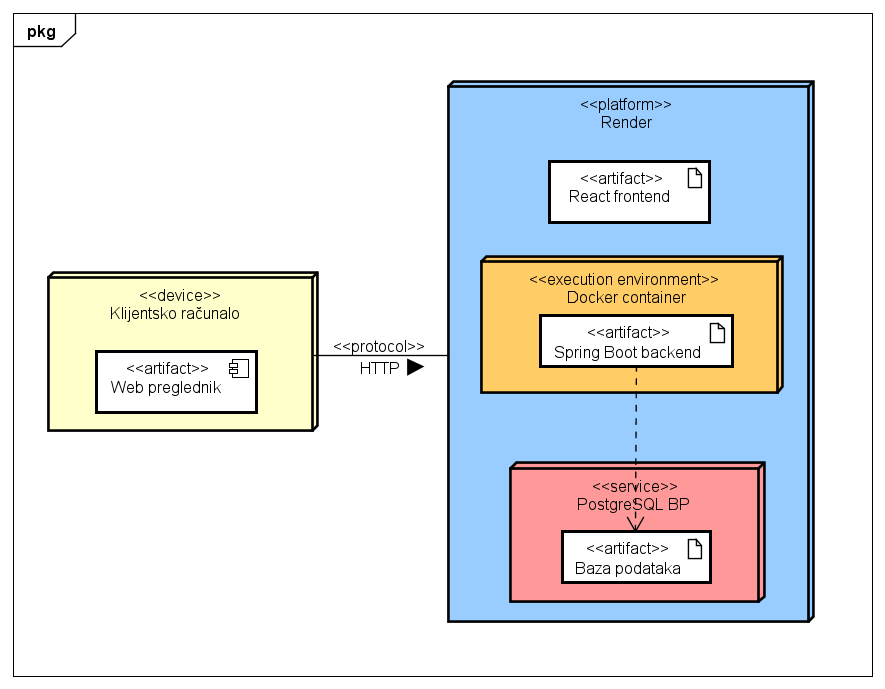
\includegraphics[scale=0.6]{slike/dijagram_razmjestaja.PNG} 
				\centering
				\caption{Dijagram razmještaja}
				\label{dijagram_razmjestaja}
			\end{figure}
			
			\eject 
		
		\section{Upute za puštanje u pogon}
		
			\textbf{\textit{dio 2. revizije}}\\
		
			 \textit{U ovom poglavlju potrebno je dati upute za puštanje u pogon (engl. deployment) ostvarene aplikacije. Na primjer, za web aplikacije, opisati postupak kojim se od izvornog kôda dolazi do potpuno postavljene baze podataka i poslužitelja koji odgovara na upite korisnika. Za mobilnu aplikaciju, postupak kojim se aplikacija izgradi, te postavi na neku od trgovina. Za stolnu (engl. desktop) aplikaciju, postupak kojim se aplikacija instalira na računalo. Ukoliko mobilne i stolne aplikacije komuniciraju s poslužiteljem i/ili bazom podataka, opisati i postupak njihovog postavljanja. Pri izradi uputa preporučuje se \textbf{naglasiti korake instalacije uporabom natuknica} te koristiti što je više moguće \textbf{slike ekrana} (engl. screenshots) kako bi upute bile jasne i jednostavne za slijediti.}
			
			
			 \textit{Dovršenu aplikaciju potrebno je pokrenuti na javno dostupnom poslužitelju. Studentima se preporuča korištenje neke od sljedećih besplatnih usluga: \href{https://aws.amazon.com/}{Amazon AWS}, \href{https://azure.microsoft.com/en-us/}{Microsoft Azure} ili \href{https://www.heroku.com/}{Heroku}. Mobilne aplikacije trebaju biti objavljene na F-Droid, Google Play ili Amazon App trgovini.}
			
			
			\eject 